\documentclass[onecolumn]{article}
%\usepackage{url}
%\usepackage{algorithmic}
\usepackage[a4paper]{geometry}
\usepackage{datetime}
\usepackage[margin=2em, font=small,labelfont=it]{caption}
\usepackage{graphicx}
\usepackage{mathpazo} % use palatino
\usepackage[scaled]{helvet} % helvetica
\usepackage{microtype}
\usepackage{amsmath}
\usepackage{subfigure}
\usepackage{hyperref}
\usepackage{graphicx}


\usepackage{listings}
\usepackage{color}
\definecolor{dkgreen}{rgb}{0,0.6,0}
\definecolor{gray}{rgb}{0.5,0.5,0.5}
\definecolor{mauve}{rgb}{0.58,0,0.82}

\lstset{frame=tb,
  language=python,
  aboveskip=3mm,
  belowskip=3mm,
  showstringspaces=false,
  columns=flexible,
  basicstyle={\small\ttfamily},
  numbers=none,
  numberstyle=\tiny\color{gray},
  keywordstyle=\color{blue},
  commentstyle=\color{dkgreen},
  stringstyle=\color{mauve},
  breaklines=true,
  breakatwhitespace=true,
  tabsize=2
}

% Letterspacing macros
\newcommand{\spacecaps}[1]{\textls[200]{\MakeUppercase{#1}}}
\newcommand{\spacesc}[1]{\textls[50]{\textsc{\MakeLowercase{#1}}}}

\title{\spacecaps{  Ceng 3007 Computer Networks Midterm }\\ \normalsize \spacesc{} }

\author{Gizem PESEN\\pesengizem@gmail.com\\
github : \textbf{https://github.com/gizempesen/ceng3007}}
%\date{\today\\\currenttime}
\date{\today}

\begin{document}
\maketitle








\section{Contents }

\begin{itemize}
\item \hyperref[sec:2]{Install packet tracer on your PC/laptop}
\item \hyperref[sec:2]{Implement the topologies}
\item \hyperref[sec:3]{Give static IP addresses to devices}
\item \hyperref[sec:4]{Ensure that these devices can make a communication }
\end{itemize}

\section{Install packet tracer on your PC/laptop}
\label{sec:2}

First, I downloaded Cisco Packet Tracker from dys.mu.edu.tr 
.\\
\begin{figure}[ht!]
\centering
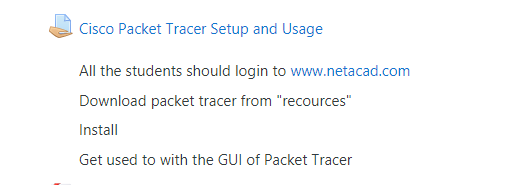
\includegraphics[width=7cm]{download.png}
\caption{Downloading place \label{}}
\end{figure}

.\\ You can clearly see the program on my desktop. I recorded screen with Apowerec.
\begin{figure}[ht!]
\centering
\includegraphics[width=7cm]{desktop.jpg}
\caption{My Desktop  \label{}}
\end{figure}

.\\\\
\section{Implement the topologies}
\label{sec:2}
This is the last view of my network. I will explain all step that I did.
.\\
\begin{figure}[ht!]
\centering
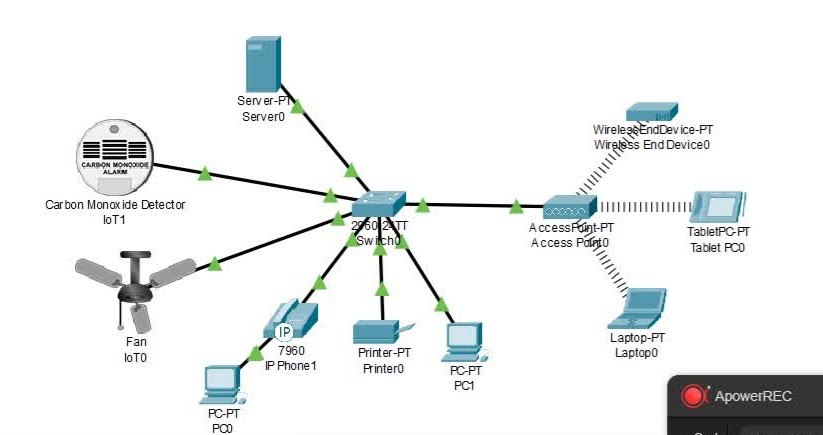
\includegraphics[width=10cm]{screenshoot.jpg}
\caption{Downloading place \label{}}
\end{figure}


\subsubsection{ Switch - Cisco 2960-24 TT}
\label{sec:2.0.1}

\begin{figure}[ht!]
\centering
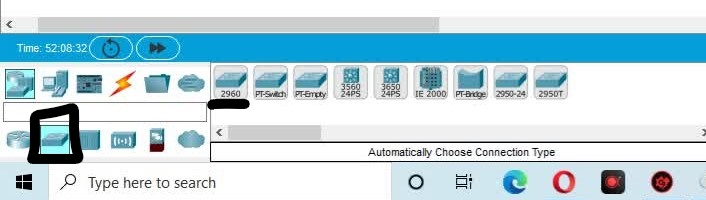
\includegraphics[width=8cm]{Inkedswitch.jpg}
\caption{Choosing switch \label{}}
\end{figure}
.\\\\

\subsubsection{Access Point}
\label{sec:2.0.2}

\begin{figure}[ht!]
\centering
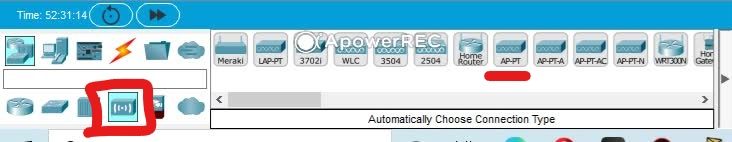
\includegraphics[width=8cm]{Inkedaccesspoint.jpg}
\caption{Choosing access point  \label{sec:2.0.2}}
\end{figure}


.\\\\\\
\subsubsection{Server}
\label{sec:2.0.3}

\begin{figure}[ht!]
\centering
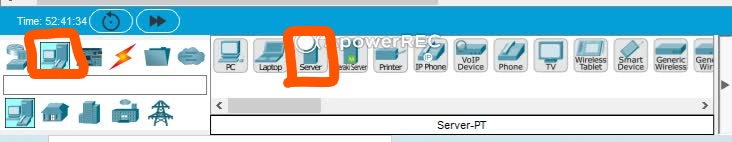
\includegraphics[width=8cm]{Inkedserver.jpg}
\caption{Choosing server \label{}}
\end{figure}



\subsubsection{IP Telephone}
\label{sec:2.0.5}

\begin{figure}[ht!]
\centering
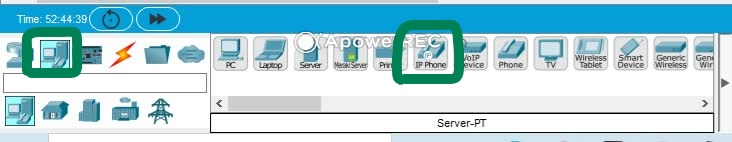
\includegraphics[width=8cm]{Inkedphone.jpg}
\caption{Choosing phone \label{sec:2.0.5}}
\end{figure}
.\\\\
I choosed Ip Phone and connected it to switch. But there was a problem and connection was not green. Because I need to change this;

\begin{figure}[ht!]
\centering
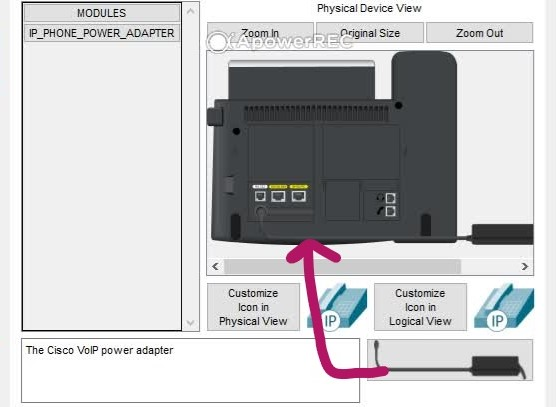
\includegraphics[width=8cm]{phoneconnection.jpg}
\caption{Choosing phone \label{}}
\end{figure}

\subsubsection{PC, Laptop, Printer, Tablet, Wireless End Device}
\label{sec:2.0.4}

It was really easy to connect 2 personal computers to our network. The\textbf{ important point} was connecting \textbf{wireless} devices. I watched a video to make \textbf{power on Laptop }device. Thanks for the hints like ;
\begin{itemize}
\item Some devices need to be “powered on” like ip phone and I learned how to.
\item Laptop needs a “wireless adapter”. and I learned how to plug it.
\end{itemize}





\begin{figure}[ht!]
\centering
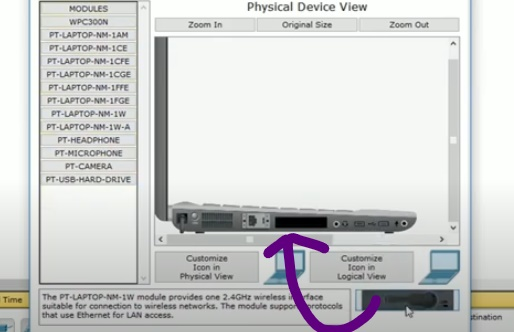
\includegraphics[width=8cm]{Inkedpoweroff.jpg}
\caption{To make active laptop \label{}}
\end{figure}


\section{Give static IP addresses to devices}
\label{sec:3}

Give static IP addresses to devices from 192.168.1.0 255.255.0 network. Fill the following table with the values in your simulation:
.\\\\\\
\begin {tabular}{crrrrl}
\hline
Device & IP Address  & Mac Address
  \\
\hline
  PC1&192.168.1.1
&0060.5C13.0438 \\
 PC0&192.168.1.2
 & 00E0.A30E.9CCD\\
 SERVER0& 192.168.1.3
&0004.9A50.8470 \\ 
 LAPTOP0& 192.168.1.4
&0060.3E0D.4486 \\  IOT0&192.168.1.5 
& 0060.470D.76CA\\  IOT1& 192.168.1.6
&00E0.8F43.95B6\\  TABLETPC1& 192.168.1.7
&0001.6458.220C\\  WIRELESSENDDEVICE0& 192.168.1.8
&0060.5C78.107A\\  PRINTER0& 192.168.1.9
&0001.42B7.E3EE
\hline
\end{tabular}
\\\\

\section{Ensure that these devices can make a communication}
\label{sec:4}

\subsubsection{Physical Layer}
\label{sec:4.0.1}

Ensure the lines are UP

\begin{figure}[ht!]
\centering
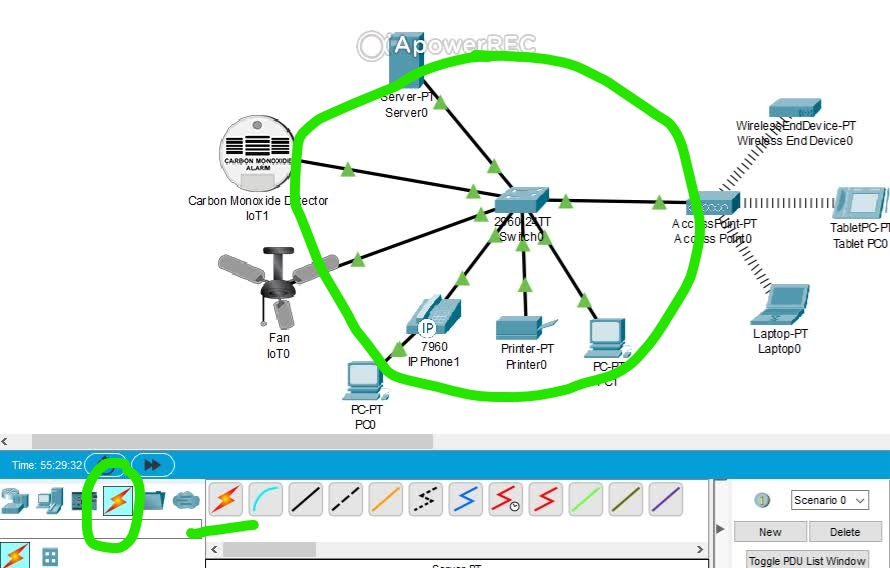
\includegraphics[width=8cm]{physicallayer.jpg}
\caption{Physical layer connection is the green cables \label{}}
\end{figure}
.\\\\


\subsubsection{Network Layer}
\label{sec:4.0.2}

Test IP based connection
\begin{figure}[ht!]
\centering
\includegraphics[width=8cm]{ipconfig.jpg}
\caption{Choosing switch \label{}}
\end{figure}
.\\\\
\begin{figure}[ht!]
\centering
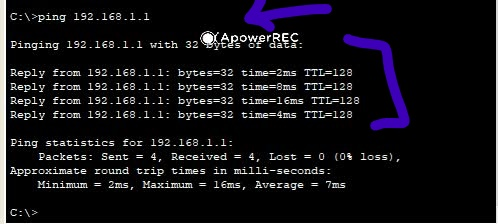
\includegraphics[width=8cm]{Inkedping.jpg}
\caption{Choosing switch \label{}}
\end{figure}
.\\\\




 
\nocite{*}
\bibliographystyle{plain}
\bibliography{references}
\end{document}
